\PassOptionsToPackage{dvipsnames,table}{xcolor}
\documentclass[10pt]{beamer}
\usepackage{Cours}

\begin{document}


\newcounter{numchap}
\setcounter{numchap}{1}
\newcounter{numframe}
\setcounter{numframe}{0}
\newcommand{\mframe}[1]{\frametitle{#1} \addtocounter{numframe}{1}}
\newcommand{\cnum}{\fbox{\textcolor{yellow}{\textbf{C\thenumchap}}}~}
\newcommand{\makess}[1]{\section{#1} \label{ss\thesection}}
\newcommand{\stitle}{\textcolor{yellow}{\textbf{\thesection. \nameref{ss\thesection}}}}

\definecolor{codebg}{gray}{0.90}
\definecolor{grispale}{gray}{0.95}
\definecolor{fluo}{rgb}{1,0.96,0.62}
\newminted[langageC]{c}{linenos=true,escapeinside=||,highlightcolor=fluo,tabsize=2,breaklines=true}
\newminted[codepython]{python}{linenos=true,escapeinside=||,highlightcolor=fluo,tabsize=2,breaklines=true}
% Inclusion complète (ou partiel en indiquant premiere et dernière ligne) d'un fichier C
\newcommand{\inputC}[3]{\begin{mdframed}[backgroundcolor=codebg] \inputminted[breaklines=true,fontsize=#3,linenos=true,highlightcolor=fluo,tabsize=2,highlightlines={#2}]{c}{#1} \end{mdframed}}
\newcommand{\inputpartC}[5]{\begin{mdframed}[backgroundcolor=codebg] \inputminted[breaklines=true,fontsize=#3,linenos=true,highlightcolor=fluo,tabsize=2,highlightlines={#2},firstline=#4,lastline=#5,firstnumber=1]{c}{#1} \end{mdframed}}
\newcommand{\inputpython}[3]{\begin{mdframed}[backgroundcolor=codebg] \inputminted[breaklines=true,fontsize=#3,linenos=true,highlightcolor=fluo,tabsize=2,highlightlines={#2}]{python}{#1} \end{mdframed}}
\newcommand{\inputpartOCaml}[5]{\begin{mdframed}[backgroundcolor=codebg] \inputminted[breaklines=true,fontsize=#3,linenos=true,highlightcolor=fluo,tabsize=2,highlightlines={#2},firstline=#4,lastline=#5,firstnumber=1]{OCaml}{#1} \end{mdframed}}
\BeforeBeginEnvironment{minted}{\begin{mdframed}[backgroundcolor=codebg]}
\AfterEndEnvironment{minted}{\end{mdframed}}
\newcommand{\kw}[1]{\textcolor{blue}{\tt #1}}

\newtcolorbox{rcadre}[4]{halign=center,colback={#1},colframe={#2},width={#3cm},height={#4cm},valign=center,boxrule=1pt,left=0pt,right=0pt}
\newtcolorbox{cadre}[4]{halign=center,colback={#1},colframe={#2},arc=0mm,width={#3cm},height={#4cm},valign=center,boxrule=1pt,left=0pt,right=0pt}
\newcommand{\myem}[1]{\colorbox{fluo}{#1}}
\mdfsetup{skipabove=1pt,skipbelow=-2pt}



% Noeud dans un cadre pour les arbres
\newcommand{\noeud}[2]{\Tr{\fbox{\textcolor{#1}{\tt #2}}}}

\newcommand{\htmlmode}{\lstset{language=html,numbers=left, tabsize=4, frame=single, breaklines=true, keywordstyle=\ttfamily, basicstyle=\small,
   numberstyle=\tiny\ttfamily, framexleftmargin=0mm, backgroundcolor=\color{grispale}, xleftmargin=12mm,showstringspaces=false}}
\newcommand{\pythonmode}{\lstset{
   language=python,
   linewidth=\linewidth,
   numbers=left,
   tabsize=4,
   frame=single,
   breaklines=true,
   keywordstyle=\ttfamily\color{blue},
   basicstyle=\small,
   numberstyle=\tiny\ttfamily,
   framexleftmargin=-2mm,
   numbersep=-0.5mm,
   backgroundcolor=\color{codebg},
   xleftmargin=-1mm, 
   showstringspaces=false,
   commentstyle=\color{gray},
   stringstyle=\color{OliveGreen},
   emph={turtle,Screen,Turtle},
   emphstyle=\color{RawSienna},
   morekeywords={setheading,goto,backward,forward,left,right,pendown,penup,pensize,color,speed,hideturtle,showturtle,forward}}
   }
   \newcommand{\Cmode}{\lstset{
      language=[ANSI]C,
      linewidth=\linewidth,
      numbers=left,
      tabsize=4,
      frame=single,
      breaklines=true,
      keywordstyle=\ttfamily\color{blue},
      basicstyle=\small,
      numberstyle=\tiny\ttfamily,
      framexleftmargin=0mm,
      numbersep=2mm,
      backgroundcolor=\color{codebg},
      xleftmargin=0mm, 
      showstringspaces=false,
      commentstyle=\color{gray},
      stringstyle=\color{OliveGreen},
      emphstyle=\color{RawSienna},
      escapechar=\|,
      morekeywords={}}
      }
\newcommand{\bashmode}{\lstset{language=bash,numbers=left, tabsize=2, frame=single, breaklines=true, basicstyle=\ttfamily,
   numberstyle=\tiny\ttfamily, framexleftmargin=0mm, backgroundcolor=\color{grispale}, xleftmargin=12mm, showstringspaces=false}}
\newcommand{\exomode}{\lstset{language=python,numbers=left, tabsize=2, frame=single, breaklines=true, basicstyle=\ttfamily,
   numberstyle=\tiny\ttfamily, framexleftmargin=13mm, xleftmargin=12mm, basicstyle=\small, showstringspaces=false}}
   
   
  
%tei pour placer les images
%tei{nom de l’image}{échelle de l’image}{sens}{texte a positionner}
%sens ="1" (droite) ou "2" (gauche)
\newlength{\ltxt}
\newcommand{\tei}[4]{
\setlength{\ltxt}{\linewidth}
\setbox0=\hbox{\includegraphics[scale=#2]{#1}}
\addtolength{\ltxt}{-\wd0}
\addtolength{\ltxt}{-10pt}
\ifthenelse{\equal{#3}{1}}{
\begin{minipage}{\wd0}
\includegraphics[scale=#2]{#1}
\end{minipage}
\hfill
\begin{minipage}{\ltxt}
#4
\end{minipage}
}{
\begin{minipage}{\ltxt}
#4
\end{minipage}
\hfill
\begin{minipage}{\wd0}
\includegraphics[scale=#2]{#1}
\end{minipage}
}
}

%Juxtaposition d'une image pspciture et de texte 
%#1: = code pstricks de l'image
%#2: largeur de l'image
%#3: hauteur de l'image
%#4: Texte à écrire
\newcommand{\ptp}[4]{
\setlength{\ltxt}{\linewidth}
\addtolength{\ltxt}{-#2 cm}
\addtolength{\ltxt}{-0.1 cm}
\begin{minipage}[b][#3 cm][t]{\ltxt}
#4
\end{minipage}\hfill
\begin{minipage}[b][#3 cm][c]{#2 cm}
#1
\end{minipage}\par
}



%Macros pour les graphiques
\psset{linewidth=0.5\pslinewidth,PointSymbol=x}
\setlength{\fboxrule}{0.5pt}
\newcounter{tempangle}

%Marque la longueur du segment d'extrémité  #1 et  #2 avec la valeur #3, #4 est la distance par rapport au segment (en %age de la valeur de celui ci) et #5 l'orientation du marquage : +90 ou -90
\newcommand{\afflong}[5]{
\pstRotation[RotAngle=#4,PointSymbol=none,PointName=none]{#1}{#2}[X] 
\pstHomO[PointSymbol=none,PointName=none,HomCoef=#5]{#1}{X}[Y]
\pstTranslation[PointSymbol=none,PointName=none]{#1}{#2}{Y}[Z]
 \ncline{|<->|,linewidth=0.25\pslinewidth}{Y}{Z} \ncput*[nrot=:U]{\footnotesize{#3}}
}
\newcommand{\afflongb}[3]{
\ncline{|<->|,linewidth=0}{#1}{#2} \naput*[nrot=:U]{\footnotesize{#3}}
}

%Construis le point #4 situé à #2 cm du point #1 avant un angle #3 par rapport à l'horizontale. #5 = liste de paramètre
\newcommand{\lsegment}[5]{\pstGeonode[PointSymbol=none,PointName=none](0,0){O'}(#2,0){I'} \pstTranslation[PointSymbol=none,PointName=none]{O'}{I'}{#1}[J'] \pstRotation[RotAngle=#3,PointSymbol=x,#5]{#1}{J'}[#4]}
\newcommand{\tsegment}[5]{\pstGeonode[PointSymbol=none,PointName=none](0,0){O'}(#2,0){I'} \pstTranslation[PointSymbol=none,PointName=none]{O'}{I'}{#1}[J'] \pstRotation[RotAngle=#3,PointSymbol=x,#5]{#1}{J'}[#4] \pstLineAB{#4}{#1}}

%Construis le point #4 situé à #3 cm du point #1 et faisant un angle de  90° avec la droite (#1,#2) #5 = liste de paramètre
\newcommand{\psegment}[5]{
\pstGeonode[PointSymbol=none,PointName=none](0,0){O'}(#3,0){I'}
 \pstTranslation[PointSymbol=none,PointName=none]{O'}{I'}{#1}[J']
 \pstInterLC[PointSymbol=none,PointName=none]{#1}{#2}{#1}{J'}{M1}{M2} \pstRotation[RotAngle=-90,PointSymbol=x,#5]{#1}{M1}[#4]
  }
  
%Construis le point #4 situé à #3 cm du point #1 et faisant un angle de  #5° avec la droite (#1,#2) #6 = liste de paramètre
\newcommand{\mlogo}[6]{
\pstGeonode[PointSymbol=none,PointName=none](0,0){O'}(#3,0){I'}
 \pstTranslation[PointSymbol=none,PointName=none]{O'}{I'}{#1}[J']
 \pstInterLC[PointSymbol=none,PointName=none]{#1}{#2}{#1}{J'}{M1}{M2} \pstRotation[RotAngle=#5,PointSymbol=x,#6]{#1}{M2}[#4]
  }

% Construis un triangle avec #1=liste des 3 sommets séparés par des virgules, #2=liste des 3 longueurs séparés par des virgules, #3 et #4 : paramètre d'affichage des 2e et 3 points et #5 : inclinaison par rapport à l'horizontale
%autre macro identique mais sans tracer les segments joignant les sommets
\noexpandarg
\newcommand{\Triangleccc}[5]{
\StrBefore{#1}{,}[\pointA]
\StrBetween[1,2]{#1}{,}{,}[\pointB]
\StrBehind[2]{#1}{,}[\pointC]
\StrBefore{#2}{,}[\coteA]
\StrBetween[1,2]{#2}{,}{,}[\coteB]
\StrBehind[2]{#2}{,}[\coteC]
\tsegment{\pointA}{\coteA}{#5}{\pointB}{#3} 
\lsegment{\pointA}{\coteB}{0}{Z1}{PointSymbol=none, PointName=none}
\lsegment{\pointB}{\coteC}{0}{Z2}{PointSymbol=none, PointName=none}
\pstInterCC{\pointA}{Z1}{\pointB}{Z2}{\pointC}{Z3} 
\pstLineAB{\pointA}{\pointC} \pstLineAB{\pointB}{\pointC}
\pstSymO[PointName=\pointC,#4]{C}{C}[C]
}
\noexpandarg
\newcommand{\TrianglecccP}[5]{
\StrBefore{#1}{,}[\pointA]
\StrBetween[1,2]{#1}{,}{,}[\pointB]
\StrBehind[2]{#1}{,}[\pointC]
\StrBefore{#2}{,}[\coteA]
\StrBetween[1,2]{#2}{,}{,}[\coteB]
\StrBehind[2]{#2}{,}[\coteC]
\tsegment{\pointA}{\coteA}{#5}{\pointB}{#3} 
\lsegment{\pointA}{\coteB}{0}{Z1}{PointSymbol=none, PointName=none}
\lsegment{\pointB}{\coteC}{0}{Z2}{PointSymbol=none, PointName=none}
\pstInterCC[PointNameB=none,PointSymbolB=none,#4]{\pointA}{Z1}{\pointB}{Z2}{\pointC}{Z1} 
}


% Construis un triangle avec #1=liste des 3 sommets séparés par des virgules, #2=liste formée de 2 longueurs et d'un angle séparés par des virgules, #3 et #4 : paramètre d'affichage des 2e et 3 points et #5 : inclinaison par rapport à l'horizontale
%autre macro identique mais sans tracer les segments joignant les sommets
\newcommand{\Trianglecca}[5]{
\StrBefore{#1}{,}[\pointA]
\StrBetween[1,2]{#1}{,}{,}[\pointB]
\StrBehind[2]{#1}{,}[\pointC]
\StrBefore{#2}{,}[\coteA]
\StrBetween[1,2]{#2}{,}{,}[\coteB]
\StrBehind[2]{#2}{,}[\angleA]
\tsegment{\pointA}{\coteA}{#5}{\pointB}{#3} 
\setcounter{tempangle}{#5}
\addtocounter{tempangle}{\angleA}
\tsegment{\pointA}{\coteB}{\thetempangle}{\pointC}{#4}
\pstLineAB{\pointB}{\pointC}
}
\newcommand{\TriangleccaP}[5]{
\StrBefore{#1}{,}[\pointA]
\StrBetween[1,2]{#1}{,}{,}[\pointB]
\StrBehind[2]{#1}{,}[\pointC]
\StrBefore{#2}{,}[\coteA]
\StrBetween[1,2]{#2}{,}{,}[\coteB]
\StrBehind[2]{#2}{,}[\angleA]
\lsegment{\pointA}{\coteA}{#5}{\pointB}{#3} 
\setcounter{tempangle}{#5}
\addtocounter{tempangle}{\angleA}
\lsegment{\pointA}{\coteB}{\thetempangle}{\pointC}{#4}
}

% Construis un triangle avec #1=liste des 3 sommets séparés par des virgules, #2=liste formée de 1 longueurs et de deux angle séparés par des virgules, #3 et #4 : paramètre d'affichage des 2e et 3 points et #5 : inclinaison par rapport à l'horizontale
%autre macro identique mais sans tracer les segments joignant les sommets
\newcommand{\Trianglecaa}[5]{
\StrBefore{#1}{,}[\pointA]
\StrBetween[1,2]{#1}{,}{,}[\pointB]
\StrBehind[2]{#1}{,}[\pointC]
\StrBefore{#2}{,}[\coteA]
\StrBetween[1,2]{#2}{,}{,}[\angleA]
\StrBehind[2]{#2}{,}[\angleB]
\tsegment{\pointA}{\coteA}{#5}{\pointB}{#3} 
\setcounter{tempangle}{#5}
\addtocounter{tempangle}{\angleA}
\lsegment{\pointA}{1}{\thetempangle}{Z1}{PointSymbol=none, PointName=none}
\setcounter{tempangle}{#5}
\addtocounter{tempangle}{180}
\addtocounter{tempangle}{-\angleB}
\lsegment{\pointB}{1}{\thetempangle}{Z2}{PointSymbol=none, PointName=none}
\pstInterLL[#4]{\pointA}{Z1}{\pointB}{Z2}{\pointC}
\pstLineAB{\pointA}{\pointC}
\pstLineAB{\pointB}{\pointC}
}
\newcommand{\TrianglecaaP}[5]{
\StrBefore{#1}{,}[\pointA]
\StrBetween[1,2]{#1}{,}{,}[\pointB]
\StrBehind[2]{#1}{,}[\pointC]
\StrBefore{#2}{,}[\coteA]
\StrBetween[1,2]{#2}{,}{,}[\angleA]
\StrBehind[2]{#2}{,}[\angleB]
\lsegment{\pointA}{\coteA}{#5}{\pointB}{#3} 
\setcounter{tempangle}{#5}
\addtocounter{tempangle}{\angleA}
\lsegment{\pointA}{1}{\thetempangle}{Z1}{PointSymbol=none, PointName=none}
\setcounter{tempangle}{#5}
\addtocounter{tempangle}{180}
\addtocounter{tempangle}{-\angleB}
\lsegment{\pointB}{1}{\thetempangle}{Z2}{PointSymbol=none, PointName=none}
\pstInterLL[#4]{\pointA}{Z1}{\pointB}{Z2}{\pointC}
}

%Construction d'un cercle de centre #1 et de rayon #2 (en cm)
\newcommand{\Cercle}[2]{
\lsegment{#1}{#2}{0}{Z1}{PointSymbol=none, PointName=none}
\pstCircleOA{#1}{Z1}
}

%construction d'un parallélogramme #1 = liste des sommets, #2 = liste contenant les longueurs de 2 côtés consécutifs et leurs angles;  #3, #4 et #5 : paramètre d'affichage des sommets #6 inclinaison par rapport à l'horizontale 
% meme macro sans le tracé des segements
\newcommand{\Para}[6]{
\StrBefore{#1}{,}[\pointA]
\StrBetween[1,2]{#1}{,}{,}[\pointB]
\StrBetween[2,3]{#1}{,}{,}[\pointC]
\StrBehind[3]{#1}{,}[\pointD]
\StrBefore{#2}{,}[\longueur]
\StrBetween[1,2]{#2}{,}{,}[\largeur]
\StrBehind[2]{#2}{,}[\angle]
\tsegment{\pointA}{\longueur}{#6}{\pointB}{#3} 
\setcounter{tempangle}{#6}
\addtocounter{tempangle}{\angle}
\tsegment{\pointA}{\largeur}{\thetempangle}{\pointD}{#5}
\pstMiddleAB[PointName=none,PointSymbol=none]{\pointB}{\pointD}{Z1}
\pstSymO[#4]{Z1}{\pointA}[\pointC]
\pstLineAB{\pointB}{\pointC}
\pstLineAB{\pointC}{\pointD}
}
\newcommand{\ParaP}[6]{
\StrBefore{#1}{,}[\pointA]
\StrBetween[1,2]{#1}{,}{,}[\pointB]
\StrBetween[2,3]{#1}{,}{,}[\pointC]
\StrBehind[3]{#1}{,}[\pointD]
\StrBefore{#2}{,}[\longueur]
\StrBetween[1,2]{#2}{,}{,}[\largeur]
\StrBehind[2]{#2}{,}[\angle]
\lsegment{\pointA}{\longueur}{#6}{\pointB}{#3} 
\setcounter{tempangle}{#6}
\addtocounter{tempangle}{\angle}
\lsegment{\pointA}{\largeur}{\thetempangle}{\pointD}{#5}
\pstMiddleAB[PointName=none,PointSymbol=none]{\pointB}{\pointD}{Z1}
\pstSymO[#4]{Z1}{\pointA}[\pointC]
}


%construction d'un cerf-volant #1 = liste des sommets, #2 = liste contenant les longueurs de 2 côtés consécutifs et leurs angles;  #3, #4 et #5 : paramètre d'affichage des sommets #6 inclinaison par rapport à l'horizontale 
% meme macro sans le tracé des segements
\newcommand{\CerfVolant}[6]{
\StrBefore{#1}{,}[\pointA]
\StrBetween[1,2]{#1}{,}{,}[\pointB]
\StrBetween[2,3]{#1}{,}{,}[\pointC]
\StrBehind[3]{#1}{,}[\pointD]
\StrBefore{#2}{,}[\longueur]
\StrBetween[1,2]{#2}{,}{,}[\largeur]
\StrBehind[2]{#2}{,}[\angle]
\tsegment{\pointA}{\longueur}{#6}{\pointB}{#3} 
\setcounter{tempangle}{#6}
\addtocounter{tempangle}{\angle}
\tsegment{\pointA}{\largeur}{\thetempangle}{\pointD}{#5}
\pstOrtSym[#4]{\pointB}{\pointD}{\pointA}[\pointC]
\pstLineAB{\pointB}{\pointC}
\pstLineAB{\pointC}{\pointD}
}

%construction d'un quadrilatère quelconque #1 = liste des sommets, #2 = liste contenant les longueurs des 4 côtés et l'angle entre 2 cotés consécutifs  #3, #4 et #5 : paramètre d'affichage des sommets #6 inclinaison par rapport à l'horizontale 
% meme macro sans le tracé des segements
\newcommand{\Quadri}[6]{
\StrBefore{#1}{,}[\pointA]
\StrBetween[1,2]{#1}{,}{,}[\pointB]
\StrBetween[2,3]{#1}{,}{,}[\pointC]
\StrBehind[3]{#1}{,}[\pointD]
\StrBefore{#2}{,}[\coteA]
\StrBetween[1,2]{#2}{,}{,}[\coteB]
\StrBetween[2,3]{#2}{,}{,}[\coteC]
\StrBetween[3,4]{#2}{,}{,}[\coteD]
\StrBehind[4]{#2}{,}[\angle]
\tsegment{\pointA}{\coteA}{#6}{\pointB}{#3} 
\setcounter{tempangle}{#6}
\addtocounter{tempangle}{\angle}
\tsegment{\pointA}{\coteD}{\thetempangle}{\pointD}{#5}
\lsegment{\pointB}{\coteB}{0}{Z1}{PointSymbol=none, PointName=none}
\lsegment{\pointD}{\coteC}{0}{Z2}{PointSymbol=none, PointName=none}
\pstInterCC[PointNameA=none,PointSymbolA=none,#4]{\pointB}{Z1}{\pointD}{Z2}{Z3}{\pointC} 
\pstLineAB{\pointB}{\pointC}
\pstLineAB{\pointC}{\pointD}
}


% Définition des colonnes centrées ou à droite pour tabularx
\newcolumntype{Y}{>{\centering\arraybackslash}X}
\newcolumntype{Z}{>{\flushright\arraybackslash}X}

%Les pointillés à remplir par les élèves
\newcommand{\po}[1]{\makebox[#1 cm]{\dotfill}}
\newcommand{\lpo}[1][3]{%
\multido{}{#1}{\makebox[\linewidth]{\dotfill}
}}

%Liste des pictogrammes utilisés sur la fiche d'exercice ou d'activités
\newcommand{\bombe}{\faBomb}
\newcommand{\livre}{\faBook}
\newcommand{\calculatrice}{\faCalculator}
\newcommand{\oral}{\faCommentO}
\newcommand{\surfeuille}{\faEdit}
\newcommand{\ordinateur}{\faLaptop}
\newcommand{\ordi}{\faDesktop}
\newcommand{\ciseaux}{\faScissors}
\newcommand{\danger}{\faExclamationTriangle}
\newcommand{\out}{\faSignOut}
\newcommand{\cadeau}{\faGift}
\newcommand{\flash}{\faBolt}
\newcommand{\lumiere}{\faLightbulb}
\newcommand{\compas}{\dsmathematical}
\newcommand{\calcullitteral}{\faTimesCircleO}
\newcommand{\raisonnement}{\faCogs}
\newcommand{\recherche}{\faSearch}
\newcommand{\rappel}{\faHistory}
\newcommand{\video}{\faFilm}
\newcommand{\capacite}{\faPuzzlePiece}
\newcommand{\aide}{\faLifeRing}
\newcommand{\loin}{\faExternalLink}
\newcommand{\groupe}{\faUsers}
\newcommand{\bac}{\faGraduationCap}
\newcommand{\histoire}{\faUniversity}
\newcommand{\coeur}{\faSave}
\newcommand{\python}{\faPython}
\newcommand{\os}{\faMicrochip}
\newcommand{\rd}{\faCubes}
\newcommand{\data}{\faColumns}
\newcommand{\web}{\faCode}
\newcommand{\prog}{\faFile}
\newcommand{\algo}{\faCogs}
\newcommand{\important}{\faExclamationCircle}
\newcommand{\maths}{\faTimesCircle}
% Traitement des données en tables
\newcommand{\tables}{\faColumns}
% Types construits
\newcommand{\construits}{\faCubes}
% Type et valeurs de base
\newcommand{\debase}{{\footnotesize \faCube}}
% Systèmes d'exploitation
\newcommand{\linux}{\faLinux}
\newcommand{\sd}{\faProjectDiagram}
\newcommand{\bd}{\faDatabase}

%Les ensembles de nombres
\renewcommand{\N}{\mathbb{N}}
\newcommand{\D}{\mathbb{D}}
\newcommand{\Z}{\mathbb{Z}}
\newcommand{\Q}{\mathbb{Q}}
\newcommand{\R}{\mathbb{R}}
\newcommand{\C}{\mathbb{C}}

%Ecriture des vecteurs
\newcommand{\vect}[1]{\vbox{\halign{##\cr 
  \tiny\rightarrowfill\cr\noalign{\nointerlineskip\vskip1pt} 
  $#1\mskip2mu$\cr}}}


%Compteur activités/exos et question et mise en forme titre et questions
\newcounter{numact}
\setcounter{numact}{1}
\newcounter{numseance}
\setcounter{numseance}{1}
\newcounter{numexo}
\setcounter{numexo}{0}
\newcounter{numprojet}
\setcounter{numprojet}{0}
\newcounter{numquestion}
\newcommand{\espace}[1]{\rule[-1ex]{0pt}{#1 cm}}
\newcommand{\Quest}[3]{
\addtocounter{numquestion}{1}
\begin{tabularx}{\textwidth}{X|m{1cm}|}
\cline{2-2}
\textbf{\sffamily{\alph{numquestion})}} #1 & \dots / #2 \\
\hline 
\multicolumn{2}{|l|}{\espace{#3}} \\
\hline
\end{tabularx}
}
\newcommand{\QuestR}[3]{
\addtocounter{numquestion}{1}
\begin{tabularx}{\textwidth}{X|m{1cm}|}
\cline{2-2}
\textbf{\sffamily{\alph{numquestion})}} #1 & \dots / #2 \\
\hline 
\multicolumn{2}{|l|}{\cor{#3}} \\
\hline
\end{tabularx}
}
\newcommand{\Pre}{{\sc nsi} 1\textsuperscript{e}}
\newcommand{\Term}{{\sc nsi} Terminale}
\newcommand{\Sec}{2\textsuperscript{e}}
\newcommand{\Exo}[2]{ \addtocounter{numexo}{1} \ding{113} \textbf{\sffamily{Exercice \thenumexo}} : \textit{#1} \hfill #2  \setcounter{numquestion}{0}}
\newcommand{\Projet}[1]{ \addtocounter{numprojet}{1} \ding{118} \textbf{\sffamily{Projet \thenumprojet}} : \textit{#1}}
\newcommand{\ExoD}[2]{ \addtocounter{numexo}{1} \ding{113} \textbf{\sffamily{Exercice \thenumexo}}  \textit{(#1 pts)} \hfill #2  \setcounter{numquestion}{0}}
\newcommand{\ExoB}[2]{ \addtocounter{numexo}{1} \ding{113} \textbf{\sffamily{Exercice \thenumexo}}  \textit{(Bonus de +#1 pts maximum)} \hfill #2  \setcounter{numquestion}{0}}
\newcommand{\Act}[2]{ \ding{113} \textbf{\sffamily{Activité \thenumact}} : \textit{#1} \hfill #2  \addtocounter{numact}{1} \setcounter{numquestion}{0}}
\newcommand{\Seance}{ \rule{1.5cm}{0.5pt}\raisebox{-3pt}{\framebox[4cm]{\textbf{\sffamily{Séance \thenumseance}}}}\hrulefill  \\
  \addtocounter{numseance}{1}}
\newcommand{\Acti}[2]{ {\footnotesize \ding{117}} \textbf{\sffamily{Activité \thenumact}} : \textit{#1} \hfill #2  \addtocounter{numact}{1} \setcounter{numquestion}{0}}
\newcommand{\titre}[1]{\begin{Large}\textbf{\ding{118}}\end{Large} \begin{large}\textbf{ #1}\end{large} \vspace{0.2cm}}
\newcommand{\QListe}[1][0]{
\ifthenelse{#1=0}
{\begin{enumerate}[partopsep=0pt,topsep=0pt,parsep=0pt,itemsep=0pt,label=\textbf{\sffamily{\arabic*.}},series=question]}
{\begin{enumerate}[resume*=question]}}
\newcommand{\SQListe}[1][0]{
\ifthenelse{#1=0}
{\begin{enumerate}[partopsep=0pt,topsep=0pt,parsep=0pt,itemsep=0pt,label=\textbf{\sffamily{\alph*)}},series=squestion]}
{\begin{enumerate}[resume*=squestion]}}
\newcommand{\SQListeL}[1][0]{
\ifthenelse{#1=0}
{\begin{enumerate*}[partopsep=0pt,topsep=0pt,parsep=0pt,itemsep=0pt,label=\textbf{\sffamily{\alph*)}},series=squestion]}
{\begin{enumerate*}[resume*=squestion]}}
\newcommand{\FinListe}{\end{enumerate}}
\newcommand{\FinListeL}{\end{enumerate*}}

%Mise en forme de la correction
\newcommand{\cor}[1]{\par \textcolor{OliveGreen}{#1}}
\newcommand{\br}[1]{\cor{\textbf{#1}}}
\newcommand{\tcor}[1]{\begin{tcolorbox}[width=0.92\textwidth,colback={white},colbacktitle=white,coltitle=OliveGreen,colframe=green!75!black,boxrule=0.2mm]   
\cor{#1}
\end{tcolorbox}
}
\newcommand{\rc}[1]{\textcolor{OliveGreen}{#1}}
\newcommand{\pmc}[1]{\textcolor{blue}{\tt #1}}
\newcommand{\tmc}[1]{\textcolor{RawSienna}{\tt #1}}


%Référence aux exercices par leur numéro
\newcommand{\refexo}[1]{
\refstepcounter{numexo}
\addtocounter{numexo}{-1}
\label{#1}}

%Séparation entre deux activités
\newcommand{\separateur}{\begin{center}
\rule{1.5cm}{0.5pt}\raisebox{-3pt}{\ding{117}}\rule{1.5cm}{0.5pt}  \vspace{0.2cm}
\end{center}}

%Entête et pied de page
\newcommand{\snt}[1]{\lhead{\textbf{SNT -- La photographie numérique} \rhead{\textit{Lycée Nord}}}}
\newcommand{\Activites}[2]{\lhead{\textbf{{\sc #1}}}
\rhead{Activités -- \textbf{#2}}
\cfoot{}}
\newcommand{\Exos}[2]{\lhead{\textbf{Fiche d'exercices: {\sc #1}}}
\rhead{Niveau: \textbf{#2}}
\cfoot{}}
\newcommand{\Devoir}[2]{\lhead{\textbf{Devoir de mathématiques : {\sc #1}}}
\rhead{\textbf{#2}} \setlength{\fboxsep}{8pt}
\begin{center}
%Titre de la fiche
\fbox{\parbox[b][1cm][t]{0.3\textwidth}{Nom : \hfill \po{3} \par \vfill Prénom : \hfill \po{3}} } \hfill 
\fbox{\parbox[b][1cm][t]{0.6\textwidth}{Note : \po{1} / 20} }
\end{center} \cfoot{}}

%Devoir programmation en NSI (pas à rendre sur papier)
\newcommand{\PNSI}[2]{\lhead{\textbf{Devoir de {\sc nsi} : \textsf{ #1}}}
\rhead{\textbf{#2}} \setlength{\fboxsep}{8pt}
\begin{tcolorbox}[title=\textcolor{black}{\danger\; A lire attentivement},colbacktitle=lightgray]
{\begin{enumerate}
\item Rendre tous vous programmes en les envoyant par mail à l'adresse {\tt fnativel2@ac-reunion.fr}, en précisant bien dans le sujet vos noms et prénoms
\item Un programme qui fonctionne mal ou pas du tout peut rapporter des points
\item Les bonnes pratiques de programmation (clarté et lisiblité du code) rapportent des points
\end{enumerate}
}
\end{tcolorbox}
 \cfoot{}}


%Devoir de NSI
\newcommand{\DNSI}[2]{\lhead{\textbf{Devoir de {\sc nsi} : \textsf{ #1}}}
\rhead{\textbf{#2}} \setlength{\fboxsep}{8pt}
\begin{center}
%Titre de la fiche
\fbox{\parbox[b][1cm][t]{0.3\textwidth}{Nom : \hfill \po{3} \par \vfill Prénom : \hfill \po{3}} } \hfill 
\fbox{\parbox[b][1cm][t]{0.6\textwidth}{Note : \po{1} / 10} }
\end{center} \cfoot{}}

\newcommand{\DevoirNSI}[2]{\lhead{\textbf{Devoir de {\sc nsi} : {\sc #1}}}
\rhead{\textbf{#2}} \setlength{\fboxsep}{8pt}
\cfoot{}}

%La définition de la commande QCM pour auto-multiple-choice
%En premier argument le sujet du qcm, deuxième argument : la classe, 3e : la durée prévue et #4 : présence ou non de questions avec plusieurs bonnes réponses
\newcommand{\QCM}[4]{
{\large \textbf{\ding{52} QCM : #1}} -- Durée : \textbf{#3 min} \hfill {\large Note : \dots/10} 
\hrule \vspace{0.1cm}\namefield{}
Nom :  \textbf{\textbf{\nom{}}} \qquad \qquad Prénom :  \textbf{\prenom{}}  \hfill Classe: \textbf{#2}
\vspace{0.2cm}
\hrule  
\begin{itemize}[itemsep=0pt]
\item[-] \textit{Une bonne réponse vaut un point, une absence de réponse n'enlève pas de point. }
\item[\danger] \textit{Une mauvaise réponse enlève un point.}
\ifthenelse{#4=1}{\item[-] \textit{Les questions marquées du symbole \multiSymbole{} peuvent avoir plusieurs bonnes réponses possibles.}}{}
\end{itemize}
}
\newcommand{\DevoirC}[2]{
\renewcommand{\footrulewidth}{0.5pt}
\lhead{\textbf{Devoir de mathématiques : {\sc #1}}}
\rhead{\textbf{#2}} \setlength{\fboxsep}{8pt}
\fbox{\parbox[b][0.4cm][t]{0.955\textwidth}{Nom : \po{5} \hfill Prénom : \po{5} \hfill Classe: \textbf{1}\textsuperscript{$\dots$}} } 
\rfoot{\thepage} \cfoot{} \lfoot{Lycée Nord}}
\newcommand{\DevoirInfo}[2]{\lhead{\textbf{Evaluation : {\sc #1}}}
\rhead{\textbf{#2}} \setlength{\fboxsep}{8pt}
 \cfoot{}}
\newcommand{\DM}[2]{\lhead{\textbf{Devoir maison à rendre le #1}} \rhead{\textbf{#2}}}

%Macros permettant l'affichage des touches de la calculatrice
%Touches classiques : #1 = 0 fond blanc pour les nombres et #1= 1gris pour les opérations et entrer, second paramètre=contenu
%Si #2=1 touche arrondi avec fond gris
\newcommand{\TCalc}[2]{
\setlength{\fboxsep}{0.1pt}
\ifthenelse{#1=0}
{\psframebox[fillstyle=solid, fillcolor=white]{\parbox[c][0.25cm][c]{0.6cm}{\centering #2}}}
{\ifthenelse{#1=1}
{\psframebox[fillstyle=solid, fillcolor=lightgray]{\parbox[c][0.25cm][c]{0.6cm}{\centering #2}}}
{\psframebox[framearc=.5,fillstyle=solid, fillcolor=white]{\parbox[c][0.25cm][c]{0.6cm}{\centering #2}}}
}}
\newcommand{\Talpha}{\psdblframebox[fillstyle=solid, fillcolor=white]{\hspace{-0.05cm}\parbox[c][0.25cm][c]{0.65cm}{\centering \scriptsize{alpha}}} \;}
\newcommand{\Tsec}{\psdblframebox[fillstyle=solid, fillcolor=white]{\parbox[c][0.25cm][c]{0.6cm}{\centering \scriptsize 2nde}} \;}
\newcommand{\Tfx}{\psdblframebox[fillstyle=solid, fillcolor=white]{\parbox[c][0.25cm][c]{0.6cm}{\centering \scriptsize $f(x)$}} \;}
\newcommand{\Tvar}{\psframebox[framearc=.5,fillstyle=solid, fillcolor=white]{\hspace{-0.22cm} \parbox[c][0.25cm][c]{0.82cm}{$\scriptscriptstyle{X,T,\theta,n}$}}}
\newcommand{\Tgraphe}{\psdblframebox[fillstyle=solid, fillcolor=white]{\hspace{-0.08cm}\parbox[c][0.25cm][c]{0.68cm}{\centering \tiny{graphe}}} \;}
\newcommand{\Tfen}{\psdblframebox[fillstyle=solid, fillcolor=white]{\hspace{-0.08cm}\parbox[c][0.25cm][c]{0.68cm}{\centering \tiny{fenêtre}}} \;}
\newcommand{\Ttrace}{\psdblframebox[fillstyle=solid, fillcolor=white]{\parbox[c][0.25cm][c]{0.6cm}{\centering \scriptsize{trace}}} \;}

% Macroi pour l'affichage  d'un entier n dans  une base b
\newcommand{\base}[2]{ \overline{#1}^{#2}}
% Intervalle d'entiers
\newcommand{\intN}[2]{\llbracket #1; #2 \rrbracket}}

% Numéro et titre de chapitre
\setcounter{numchap}{0}
\newcommand{\Ctitle}{\cnum Notions d'architecture et de système}

\makess{Architecture des ordinateurs}
\begin{frame}{\Ctitle}{\stitle}
	\begin{block}{Modèle de Von Neumann}
		\begin{itemize}
			\item<1-> Les ordinateurs modernes sont construits autour d'un modèle défini par le mathématicien John Von Neumann dans les années 1940 appelé \textcolor{blue}{Architecture de Von Neumann}
			\item<2-> Dans ce modèle, l'ordinateur se décompose :
				\begin{itemize}
					\item<3-> La \textcolor{blue}{mémoire} qui stocke les données et les programmes (sous forme de 0 et de 1).
					\item<4-> L'\textcolor{blue}{unité arithmétique et logique {\sc ual}} qui effectue les opérations arithmétiques (addition, soustraction, \dots) et logiques (conjonctions, négations, \dots) sur les données.
					\item<5-> L'\textcolor{blue}{unité de contrôle} chargé de l'ordre des opérations et de la récupération des données en mémoire.
					\item<6-> Les dispositifs d'\textcolor{blue}{entrée} (ex : clavier, souris, réseau, \dots), et de \textcolor{blue}{sortie} (ex : écran, imprimante, \dots) des données
				\end{itemize}
		\end{itemize}
	\end{block}
\end{frame}


\begin{frame}{\Ctitle}{\stitle}
	
	\begin{block}{Schéma représentant l'architecture de Von Neumann :}
		\rnode{cmp}{\psframe[linewidth=0.8pt,linecolor=Sepia](3.2,0)(8.8,-5)}
		\rput(6,-1.4){\rnode{cpu}{\psshadowbox[shadowsize=1pt,framesep=0.5cm]{\makebox[4cm]{\raisebox{1cm}{\textcolor{BrickRed}{\textbf{\faMicrochip \ CPU}} } } }}}
		\onslide<2->{\rput(4.5,-1.8){\rnode{ual}{\psframebox[framearc=.3,framesep=0.2cm,linewidth=0.4pt]{\makebox[1.2cm]{UAL}}}}}
		\onslide<2->{\rput(7.5,-1.8){\rnode{uc}{\psframebox[framearc=.3,framesep=0.2cm,linewidth=0.4pt]{\makebox[1.2cm]{UC}}}}}
		\onslide<3->{\rput(5.75,-4.2){\rnode{ram}{\psshadowbox[shadowsize=1pt,framesep=0.5cm]{\makebox[4cm]{\textcolor{BrickRed}{\textbf{\faMemory \ Mémoire}}} }}}}
		\onslide<4->{\rput(0.8,-2.4){\rnode{in}{\psshadowbox[shadowsize=1pt,framesep=0.4cm]{\makebox[1.2cm]{\textcolor{blue}{\textbf{Entrées \ \faArrowAltCircleRight}}} }}}}
		\onslide<5->{\rput(10.4,-2.4){\rnode{out}{\psshadowbox[shadowsize=1pt,framesep=0.4cm]{\makebox[1.2cm]{\textcolor{blue}{\textbf{\faArrowAltCircleRight \ Sorties}}} }}}}
		\onslide<6->{\ncline[linecolor=blue, linewidth=2px, offset = 1.5cm]{<->}{ram}{cpu}
			\ncline[linecolor=blue, linewidth=2px, offset = -1.5cm]{<->}{ram}{cpu}}
		\onslide<7->{\ncline[linecolor=blue, linewidth=2px,offsetA=-0.2cm,offsetB=-0.37cm,nodesepB=0.4cm]{->}{in}{cpu}
			\ncline[linecolor=blue, linewidth=2px,offsetB=-0.17cm,offsetA=-0.35cm,nodesepA=0.3cm]{->}{cpu}{out}}
		\vspace{5cm}
	\end{block}
\end{frame}

\makess{Système d'exploitation}
\begin{frame}{\Ctitle}{\stitle}	
	\begin{alertblock}{Définition}
		Un \textcolor{red}{système d'exploitation}  (en abrégé \textcolor{red}{OS}, de l'anglais \textit{Operating System}) est un programme (ou ensemble de programme) permettant de
		\onslide<2->{gérer les ressources de l'ordinateur (mémoire, fichier, périphériques, \dots) sur lequel il s'execute}. \\
	\end{alertblock}
	\onslide<3->{\begin{exampleblock}{Exemples}
			Les systèmes d'exploitation les plus répandus à l'heure actuelle sont :
			\begin{itemize}
				\item[\faWindows] <4-> Windows (différentes versions)
				\item[\faLinux] <5-> {\sc gnu}/Linux  (plusieurs centaines de distribution différentes, parmi les plus connus : ubuntu, fedora, archlinux)
				\item[\faAndroid] <6-> Android (smartphone)
				\item[\faApple] <7-> MacOs (ordinateur) et iOS (smartphone)
			\end{itemize}
		\end{exampleblock}}
\end{frame}

%Schéma représentatif
\begin{frame}{\Ctitle}{\stitle}
	\begin{block}{La place du système d'exploitation}
		\setlength{\shadowsize}{1pt}
		\begin{tabularx}{0.9\textwidth}{Y}
			\onslide<2->{\rnode{ut}{\psshadowbox{\makebox[5cm]{\par\noindent\rule[-0.2cm]{0pt}{0.6cm} \textcolor{BrickRed}{\textbf{\faUser \ L'utilisateur}} }} } }           \\
			\\
			\onslide<3->{\rnode{ap}{\psshadowbox{\makebox[5cm]{\par\noindent\rule[-0.2cm]{0pt}{0.6cm} {\textcolor{BrickRed}{\textbf{\faThList \ Les applications}} } }}}}     \\
			\\
			\onslide<6->{\rnode{os}{\psshadowbox{\makebox[5cm]{\par\noindent\rule[-0.2cm]{0pt}{0.6cm} {\textcolor{BrickRed}{\textbf{\faLinux \ Système d'exploitation}}} }}}} \\
			\\
			\onslide<6->{\rnode{or}{\psshadowbox{\makebox[5cm]{\par\noindent\rule[-0.2cm]{0pt}{0.6cm} {\textcolor{BrickRed}{\textbf{\faLaptop \ L'ordinateur}}} }}}}
		\end{tabularx}
		\onslide<4->{\ncline[doubleline=true,offset=1cm,doublesep=3pt,doublecolor=blue,linecolor=blue,linewidth=0.5pt,arrowsize=10pt,arrowinset=0.2,arrowlength=1.2]{->}{ut}{ap}}
		\onslide<4->{\ncline[doubleline=true,offset=1.5cm,doublesep=3pt,doublecolor=blue,linecolor=blue,linewidth=0.5pt,arrowsize=10pt,arrowinset=0.2,arrowlength=1.2]{<-}{ut}{ap}}
		\onslide<5->{\naput{ \textit{\small interagit avec} }}
		\onslide<7->{\ncline[doubleline=true,offset=0cm,doublesep=3pt,doublecolor=blue,linecolor=blue,linewidth=0.5pt,arrowsize=10pt,arrowinset=0.2,arrowlength=1.2]{<-}{ap}{os}}
		\onslide<7->{\ncline[doubleline=true,offset=0.5cm,doublesep=3pt,doublecolor=blue,linecolor=blue,linewidth=0.5pt,arrowsize=10pt,arrowinset=0.2,arrowlength=1.2]{->}{ap}{os}}
		\onslide<7->{\naput{\textit{\small demandent des ressources au}}}
		\onslide<8->{\ncline[doubleline=true,offset=-1cm,doublesep=3pt,doublecolor=blue,linecolor=blue,linewidth=0.5pt,arrowsize=10pt,arrowinset=0.2,arrowlength=1.2]{<-}{os}{or}}
		\onslide<8->{\ncline[doubleline=true,offset=-0.5cm,doublesep=3pt,doublecolor=blue,linecolor=blue,linewidth=0.5pt,arrowsize=10pt,arrowinset=0.2,arrowlength=1.2]{->}{os}{or}}
		\onslide<8->{\naput{\textit{\small gèrent les ressources de		}}}
	\end{block}
\end{frame}

\begin{frame}{\Ctitle}{\stitle}
	\begin{block}{Fonctionnalités d'un système d'exploitation}
		\begin{itemize}
			\item<1-> Gestion des périphériques.
			\item<2-> Donner l'illusion que l'ordinateur est multitâches.
			\item<3-> Gérer les différentes applications utilisées.
			\item<4-> Identifier les utilisateurs.
			\item<5-> Contrôler et distribuer les accès aux ressources de l'ordinateur.
			\item<6-> Gérer le système de fichier.
		\end{itemize}
	\end{block}
\end{frame}

\begin{frame}{\Ctitle}{\stitle}	
	\begin{block}{Le système de gestion de fichiers}
		\begin{itemize}
			\item<1-> L'ensemble des fichiers forme une arborescence démarrant au répertoire \textcolor{Sepia}{\tt /} appelé \textcolor{blue}{racine} (\textit{root}) \hspace{-2cm}.
				\onslide<2->{\pstree[levelsep=0.8cm]{\noeud{blue}{/}}{
						\pstree[levelsep=0.8cm]{\noeud{blue}{bin}}{\Tr{\textcolor{Sepia}{\tt ls}} \Tr{\textcolor{Sepia}{\tt cat}}}
						\noeud{blue}{etc}
						\noeud{blue}{tmp}
						\pstree[levelsep=1cm]{\noeud{blue}{home}}{\noeud{blue}{\footnotesize Pierre} \noeud{blue}{\footnotesize Paul} \noeud{blue}{\footnotesize Jacques}}}}
			\item<3-> Les fichiers où les répertoires sont spécifiés :
				\begin{itemize}
					\item<4-> s'ils commencent par \textcolor{blue}{\tt /} en chemin \textcolor{blue}{absolu} c'est à dire depuis la racine.
					\item<5-> sinon en chemin \textcolor{blue}{relatif} c'est à dire depuis le répertoire courant (le répertoire parent se note alors \textcolor{blue}{\tt ..}).
				\end{itemize}
			\item<6-> Trois type de droits sont définis sur les fichiers et dossiers :
				\begin{itemize}
					\item<6->[{\tt r}] droit de lecture du fichier
					\item<7->[{\tt w}] droit d'écriture  dans le fichier
					\item<8->[{\tt x}] droit d'execution du fichier
				\end{itemize}
		\end{itemize}
	\end{block}
\end{frame}

\makess{Le \textit{shell}}
\begin{frame}{\Ctitle}{\stitle}
	\begin{block}{Interface système : \textit{shell}}
		\begin{itemize}
			\item<1-> Avant l'avènement des interfaces graphiques (et de la souris), l'utilisateur communiquait avec le système d’exploitation via un programme appelé \textcolor{blue}{\textit{shell}} par l'intermédiaire d'un simple clavier et d'une interface en ligne de commande ({\sc cli} en anglais pour \textit{Command Line Interface}).
			\item<2-> Aujourd'hui encore et pour diverses raisons (rapidité, contrôle plus fin de l'ordinateur, récupération d'erreurs, \dots) la ligne de commande reste très utilisée.
			\item<3-> Voici un exemple d'invite de commande :\\
				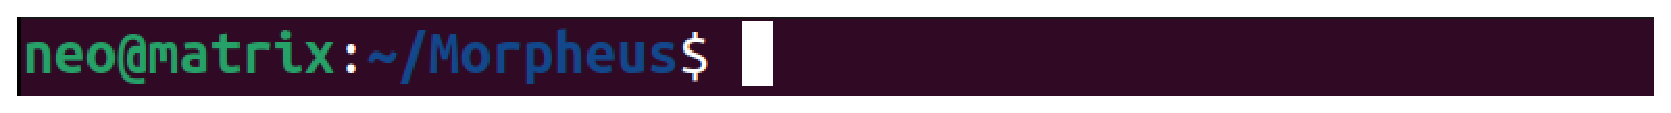
\includegraphics[width=200px]{neo.eps} \\
				On y trouve :
				\begin{itemize}
					\item<4-> Le nom de l'utilisateur ici \textcolor{green}{\tt neo} suivi de \textcolor{green}{\tt @}
					\item<5-> Le nom de l'ordinateur ici \textcolor{green}{\tt matrix} suivi de {\tt :}
					\item<6-> Le chemin du dossier de travail ici \textcolor{blue}{\tt \~{}/Morpheus}  suivi de {\tt :} et du curseur
				\end{itemize}
		\end{itemize}
	\end{block}
\end{frame}

\begin{frame}{\Ctitle}{\stitle}
	\begin{block}{Généralités sur le {\tt shell}}
		\begin{itemize}
			\item<1-> Les commandes ont généralement le format suivant : \\
				\textcolor{blue}{\tt <nom commande> <option> <arguments>} \\
				où les options sont précédées d'un tiret  simple \textcolor{Sepia}{\tt -} ou double \textcolor{Sepia}{\tt -{}-}
			\item<2-> certains caractères spéciaux permettent d'agir sur un ensemble d'arguments : \\
				\begin{tabularx}{0.8\linewidth}{|c|X|}
					\hline
					\textcolor{Sepia}{\tt ?}    & correspond à n'importe quel caractère                      \\
					\hline
					\textcolor{Sepia}{\tt *}    & correspond à n'importe quel suite de caractères            \\
					\hline
					\textcolor{gray}{\tt [...]} & \textcolor{gray}{correspond aux caractères entre crochets} \\
					\hline
				\end{tabularx}
			\item<3-> Le résultat d'une commande peut-être dirigé :
				\begin{itemize}
					\item<4-> Vers un fichier avec \textcolor{Sepia}{\tt >} (avec écrasement si le fichier existe)
					\item<5-> Vers un fichier avec \textcolor{Sepia}{\tt >{}>} (avec ajout en fin si le fichier existe)
					\item<6-> Vers une autre commande avec \textcolor{Sepia}{\tt |} (\textit{pipe})
				\end{itemize}
		\end{itemize}
	\end{block}
\end{frame}

\begin{frame}{\Ctitle}{\stitle}
	\begin{block}{Quelques commandes}
		\begin{description}
			\item<1->[\textcolor{blue}{\tt man}] : affiche l'aide sur une commande
			\item<2->[\textcolor{blue}{\tt pwd}] : affiche le répertoire courant
			\item<3->[\textcolor{blue}{\tt mkdir}] : crée un ou plusieurs dossiers
			\item<4->[\textcolor{blue}{\tt rmdir}] : supprime un dossier
			\item<5->[\textcolor{blue}{\tt mv}] : déplace un dossier ou un fichier
			\item<6->[\textcolor{blue}{\tt ls}] : liste le contenu d'un dossier
				{\footnotesize \begin{itemize}
						\item[{\tt -a}] affiche les fichiers cachés (dont le nom commence par un point)
						\item[{\tt -l}] permet de voir les droits sur les fichiers
						\item[{\tt -i}] permet de voir les inodes
					\end{itemize}}
			\item<7->[\textcolor{blue}{\tt cat}] : écrit le contenu d'un fichier dans le terminal
			\item<8->[\textcolor{blue}{\tt touch}] : crée un fichier vide
			\item<9->[\textcolor{blue}{\tt echo}] : écrit dans le terminal
			\item<10->[\textcolor{blue}{\tt cp}] : copie un fichier
		\end{description}
	\end{block}
\end{frame}

\begin{frame}{\Ctitle}{\stitle}
	\begin{exampleblock}{Exemples}
		\tei{ExArbo.eps}{0.4}{1}{
		A partir du répertoire {\tt Cours}, écrire les commandes pour :
		\begin{enumerate}
			\item<1-> Créer le fichier vide {\tt to\_do} \\
				\onslide<2->{\textcolor{OliveGreen}{\tt touch to\_do}}
			\item<3-> Ecrire dans ce fichier : "{\tt réviser le chapitre 0}" \\
				\onslide<4->{\textcolor{OliveGreen}{\tt echo "réviser le chapitre 0" > to\_do}}
			\item<5-> se déplacer vers le dossier {\tt Factures} (chemin relatif)\\
				\onslide<6->{\textcolor{OliveGreen}{{\tt cd ../../Documents/Factures}}}
			\item<7-> y créer les dossiers {\tt Eau}, {\tt Electricité} et {\tt Téléphone}\\
				\onslide<8-> {\textcolor{OliveGreen}{{\tt mkdir Eau Electricité Téléphone}}}
			\item<9-> lister tous le fichiers contenant {\tt edf}\\
				\onslide<10-> {\textcolor{OliveGreen}{{\tt ls *edf*}}}
			\item<11-> Les déplacer dans le dossier {\tt Electricité}\\
				\onslide<12-> {\textcolor{OliveGreen}{{\tt mv *edf* Electricité}}}
		\end{enumerate}
		}
	\end{exampleblock}
\end{frame}

\begin{frame}{\Ctitle}{\stitle}
	\begin{block}{Droits sur un fichier, {\tt chmod}}
		\begin{itemize}
			\item<2-> Les droits sur un fichier (\textcolor{blue}{\tt r} : lecture, \textcolor{blue}{\tt w} : écriture, \textcolor{blue}{\tt x} exécution) sont définis pour le propriétaire : {\textcolor{blue}{\tt u}} (\textit{user}), le groupe : {\textcolor{blue}{\tt g}} (\textit{groupe}) et les autres :{\textcolor{blue}{\tt o}} (\textit{others}).
			\item<3-> La commande \textcolor{blue}{\tt ls -l} permet d'afficher les droits, par exemple : \\
				{\tt rwxr-x---} indique que l'utilisateur a tous les droits, le groupe peut lire et écrire et les autres n'ont aucun droit.
			\item<4-> La commande \textcolor{blue}{\tt chmod} permet de modifier les droits, à l'aide de {\tt +} (ajout), {\tt -} (retrait), {\tt =} (attribution) ou en notation octale ({\tt r=4, w=2, x=1}).
		\end{itemize}
	\end{block}
	\begin{exampleblock}{Exemples}
		\begin{itemize}
			\item<5->{{\tt chmod u+w } :} \onslide<6->{\footnotesize Ajoute  ({\tt +}) le droit d'écriture ({\tt w}) au propriétaire ({\tt g}) }
			\item<7->{{\tt chmod 700 } :} \onslide<8->{\footnotesize Le propriétaire a tous les droits, les autres et le groupe aucun}
			\item<9->{{\tt chmod og-r } :} \onslide<10->{\footnotesize Enlève ({\tt -}) le droit de lecture ({\tt r}) au groupe et aux autres ({\tt og}) }
			\item<11->{{\tt chmod 544} :} \onslide<12->{\footnotesize Le propriétaire peut lire et exécuter, le groupe et les autres peuvent lire}
		\end{itemize}
	\end{exampleblock}
\end{frame}

\makess{Liens et inodes}
\begin{frame}{\Ctitle}{\stitle}
	\begin{block}{Liens physiques ou symboliques}
		\begin{itemize}
			\item<1-> Les fichiers sont stockés sur le support physique par blocs et retrouvés grâce à leur \textcolor{blue}{inode} (\textit{index node} ou noeud d'index).
			\item<2-> Deux noms de fichiers différents peuvent référencer les mêmes données, ils partagent alors le même inode, on dit que c'est un lien physique (\textit{hardlink}).
			\item<3-> Un lien symbolique (\textit{softlink}) est un fichier indiquant un chemin vers un autre fichier (équivalent d'un raccourci de \textit{Windows}).
			\item<4-> La commande \textcolor{blue}{\tt ln} (resp. \textcolor{blue}{\tt ln -s}) permet de créer un lien physique (resp. symbolique).
		\end{itemize}
	\end{block}
	\begin{exampleblock}{Exemples}
		\begin{itemize}
			\item<5-> {\tt ln important.txt ../Sauvegarde/important.sav} \\
				\onslide<6->{Les deux noms de fichiers font référence aux mêmes données}
			\item<7-> {\tt ln -s important.txt ../Sauvegarde/important.sav} \\
				\onslide<8->{Création d'une simple redirection}
		\end{itemize}
	\end{exampleblock}
\end{frame}

\end{document}
